\documentclass{beamer}
\usepackage{up}

\title{Рекурсия}

\date[21.12.16 г. -- 4.01.17 г.]{21 декември 2016 г. -- 4 януари 2017 г.}

\usetikzlibrary{arrows.meta}

\begin{document}

\begin{frame}
  \titlepage
\end{frame}

\section{Какво е рекурсия?}

\begin{frame}
  \frametitle{Какво е рекурсия?}

  \begin{center}
    \temporal<2>{
      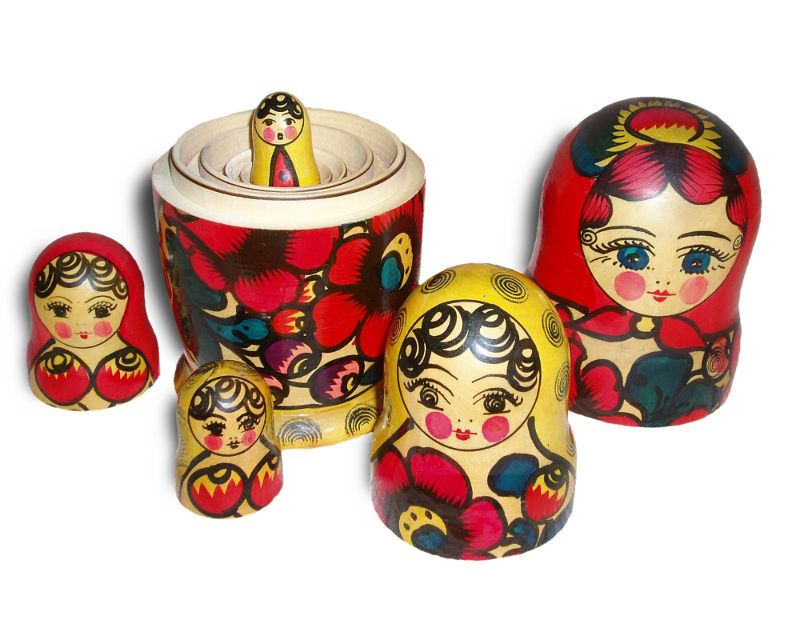
\includegraphics[width=.8\textwidth]{images/matroska.jpg}
    }{
      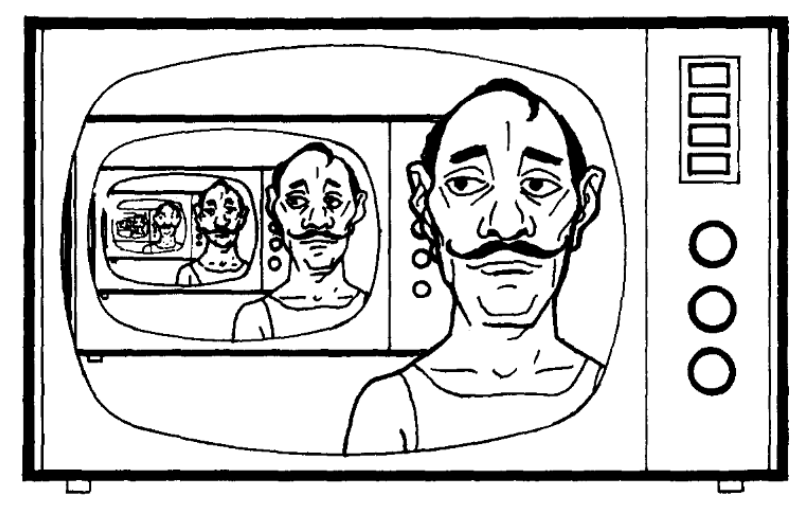
\includegraphics[width=.8\textwidth]{images/knuth.png}\\
      \imgcite{N. Wirth, Algorithms and Data Structures, Fig 3.1}
    }{ \only<3>{
        \vspace{5em}
        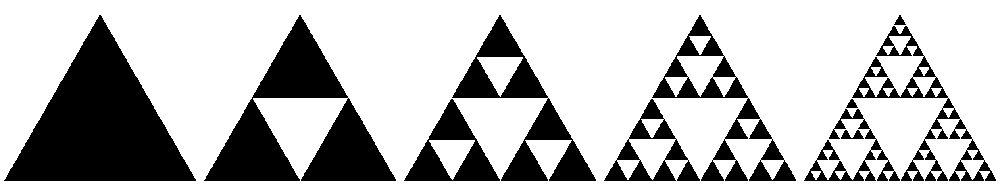
\includegraphics[width=.8\textwidth]{images/sierpinski.png}
      }}
  \end{center}
  \begin{itemize}[<+(3)->]
  \item Повторение чрез позоваване на себе си
  \item ``приятелите на моите приятели са и мои приятели''
  \item директориите съдържат файлове и директории
  \item PHP = PHP Hypertext preprocessor
  \item за да строшите камък:
    \begin{itemize}
    \item ударете с чука, за да натрошите камъка на части
    \item строшете получените по-малки камъни
    \end{itemize}
  \item за да разберете какво е рекурсия, трябва да разберете какво е рекурсия
  \end{itemize}
\end{frame}

\begin{frame}
  \frametitle{Рекурсията в математиката}

  \begin{equation*}
    n! =
    \begin{cases}
      1,& n = 0,\\
      n(n-1)!,&n > 0.
    \end{cases}
  \end{equation*}
  \pause
  \begin{equation*}
    x^n =
    \begin{cases}
      1,&n = 0,\\
      x.x^{n-1},&n > 0,\\
      \frac1{x^{-n}},&n<0.
    \end{cases}
  \end{equation*}
  \pause
  \begin{equation*}
    gcd(a,b)=
    \begin{cases}
      a,&a = b,\\
      gcd(a-b,b),&a>b,\\
      gcd(a,b-a),&a<b.
    \end{cases}
  \end{equation*}
  \pause
  \begin{equation*}
    f(x)=
    \begin{cases}
      0,&x = 0,\\
      f(x+1)-1,&x>0.
    \end{cases}
  \end{equation*}
\end{frame}

\begin{frame}
  \frametitle{Как се решават задачи с рекурсия?}

  \begin{itemize}[<+->]
  \item \alert{Декомпозиция} --- свеждане на дадена задача към множество от по-прости задачи
  \item Рекурсията е вид декомпозиция, при който свеждаме задача към множество от по-прости задачи \alert{подобни на първоначалната}
  \item Как работи:
    \begin{itemize}
    \item Показваме решението на най-простите задачи \alert{(база, дъно)}
    \item Показваме как по-сложна задача се свежда към една или няколко по-прости \alert{(стъпка)}
    \end{itemize}
  \end{itemize}
\end{frame}

\begin{frame}
  \frametitle{Математическа индукция}

  \begin{definition}
    \textbf{Математическата индукция} е метод за доказателство, използващ като предпоставка свойството, което се доказва.
  \end{definition}
  \pause
  \textbf{Пример:} Да се докаже, че $2 + 4 + ... + 2n = n(n+1)$.\\[1em]
  \pause
  \textbf{Доказателство:}
  \begin{itemize}[<+->]
  \item за $n = 0$: трябва да проверим, че $0 = 0.1\quad\checkmark$
  \item нека допуснем, че сме доказали свойството за дадено $n$
  \item ще го докажем за $n+1$:
  \item $(2 + 4 + ... + 2n) + 2(n+1) = n(n+1) + 2(n+1) = (n+1)(n+2)\quad\checkmark$
  \item \textbf{Следователно:} доказахме свойството за произволно $n$. $\qed$
  \end{itemize}
  \onslide<+->
  Математическата индукция е рекурсивен метод за доказателство.
\end{frame}

\section{Рекурсивни програми}

\begin{frame}
  \frametitle{Рекурсията в програмирането}

  \begin{definition}
    \textbf{Рекурсивна функция} наричаме функция, която извиква себе си пряко или косвено.
  \end{definition}
  \pause
  \vspace{2em}
  Рекурсивни функции се поддържат от почти всички съвременни езици за програмиране.\\[2em]
  \pause
  \begin{theorem}
    Всяка програма с цикли може да се напише с рекурсия и обратно.
  \end{theorem}
\end{frame}

\begin{frame}<1>
  \frametitle{Примери за рекурсивни функции}

  Да се напише функция, която пресмята рекурсивно:
  \begin{enumerate}[<+->]
  \item $n!$
  \item НОД
  \item $x^n$
  \item числата на Фибоначи
  \item числата на Фибоначи, но \alert{по-бързо}.
  \item{} <израз> със скоби, където
    \begin{itemize}[<.->]
    \item{} <израз> ::= <цифра> | \tta(<израз><операция><израз>\tta)
    \item{} <цифра> ::= \tta0 | \tta1 | \tta2 | \tta3 | \tta4 | \tta5 | \tta6 | \tta7 | \tta8 | \tta9
    \item{} <операция> ::= \tta+ | \tta- | \tta* | \tta/
    \end{itemize}
  \end{enumerate}
\end{frame}

\begin{frame}<1-11>[label=current]
  \frametitle{Стекови рамки на рекурсивни функции}

    \tikzset{
    m/.style={
      matrix of nodes,
      nodes={
        text height=1ex,
        text depth=0.25ex,
        minimum height=1em,
        minimum width=8ex
      },
      nodes in empty cells,
      ampersand replacement=\&
    },
    table/.style={
      rectangle,
      very thin,
      minimum width=25ex,
      fill=diagramblue,
      draw=black
    }
  }

  \begin{center}
    \begin{tikzpicture}
      \matrix [m,
         row 1/.style={row 2},row 2/.style={visible on=<6>},
         row 3/.style={row 4},row 4/.style={visible on=<5-7>},
         row 5/.style={row 6},row 6/.style={visible on=<4-8>},
         row 7/.style={row 8},row 8/.style={visible on=<3-9>},
         row 9/.style={row 10},row 10/.style={visible on=<2-10>}] {
       |(fact0)| \tt{fact} \& \& |(r0) [table]| адрес на връщане \& \lst{return 1;}\\
       \& \tt{n} \& |(n0) [table]| 0 \& \\
       |(fact1)| \tt{fact} \& \& |(r1) [table]| адрес на връщане \& \alt<-6>{\lst{return 1 * fact(0);}}{\lst{return 1 * 1;}}\\
       \& \tt{n} \& |(n1) [table]| 1 \& \\
       |(fact2)| \tt{fact} \& \& |(r2) [table]| адрес на връщане \& \alt<-7>{\lst{return 2 * fact(1);}}{\lst{return 1 * 2;}}\\
       \& \tt{n} \& |(n2) [table]| 2 \& \\
       |(fact3)| \tt{fact} \& \& |(r3) [table]| адрес на връщане \& \alt<-8>{\lst{return 3 * fact(2);}}{\lst{return 3 * 2;}}\\
       \& \tt{n} \& |(n3) [table]| 3 \& \\
       |(fact4)| \tt{fact} \& \& |(r4) [table]| адрес на връщане \& \alt<-9>{\lst{return 4 * fact(3);}}{\lst{return 4 * 6;}}\\
       \& \tt{n} \& |(n4) [table]| 4 \& \\
       |(main)| \tt{main} \& \tt n \& |(nmain) [table]| 4 \& \alt<-10>{\lst{cout << fact(4);}}{\lst{cout << 24;}}\\
      };
      \foreach \i in {0,...,4} { 
        \FPeval{from}{clip(6-\i)}
        \FPeval{to}{clip(6+\i)}
        \draw[very thick, draw on=<\from-\to>] (fact\i.north west) -- (r\i.north west) rectangle (n\i.south east);
      }
      \draw[very thick] (main.north west) -- (nmain.north west) rectangle (nmain.south east);
    \end{tikzpicture}
  \end{center}

\end{frame}

\begin{frame}
  \frametitle{Рекурсивни функции за масиви}

  Да се напише функция, която чрез рекурсия
  \begin{enumerate}[<+->]
  \item намира сума на елементите на масив
  \item проверява дали елемент съществува в масив
  \item проверява дали елементите на масив са подредени в растящ ред
  \item проверява дали елементите на масив са различни
  \item сортира масив с алгоритъма за ``бързо сортиране''
  \end{enumerate}
\end{frame}

\begin{frame}
  \frametitle{Алгоритъм за бързо сортиране}

  \begin{enumerate}[<+->]
  \item Избираме елемент от масива (``ос'')
  \item Разделяме масива на две части:
    \begin{itemize}
    \item елементи по-малки от оста
    \item елементи по-големи или равни на оста
    \end{itemize}
  \item поставяме оста между двете части на масива
  \item \alert{рекурсивно} сортираме поотделно двете части на масива
  \end{enumerate}
  \onslide<+->
  Този подход за решение се нарича ``разделяй и владей''.
\end{frame}

\section{Търсене с връщане назад}

\begin{frame}
  \frametitle{Задачи за търсене}

  Видове задачи за търсене:
  \begin{itemize}[<+->]
  \item директно изброяване на кандидатите за решение
    \begin{itemize}
    \item имаме предварително зададена последователност за обработка на всички случаи
    \item \textbf{Примери:} търсене на елемент в масив, търсене на число с дадено свойство
    \end{itemize}
  \item построяване на частични кандидати за решение
    \begin{itemize}
    \item нямаме ясна последователност за обработка на случаите
    \item \textbf{Примери: } търсене на път в лабиринт, решаване на Судоку, игра на шах
    \end{itemize}
  \end{itemize}
\end{frame}

\begin{frame}
  \frametitle{Търсене с връщане назад (backtracking)}

  Търсене с \alert{проба и грешка}:
  \begin{itemize}[<+->]
  \item започваме от началната позиция
  \item кои са вариантите да продължим напред?
    \begin{itemize}
    \item няколко са, правим \textbf{избор} на един от тях \alert{(проба, стъпка напред)}
    \item няма такива, отказваме се от текущия вариант и се \textbf{връщаме} да коригираме последния направен избор \alert{(грешка, стъпка назад)}
    \end{itemize}
  \item ако намерим търсеното решение: \alert{успех!}
  \item ако изчерпим всички варианти: \alert{провал!}
  \end{itemize}
\end{frame}

\begin{frame}
  \frametitle{Пример: търсене на път в лабиринт}

  \textbf{Задача.} Матрица от символи представя правоъгълен лабиринт:
  \begin{itemize}
  \item \tt\textvisiblespace\ --- празна клетка
  \item \tt* --- стена
  \item \tt\$ --- съкровище
  \end{itemize}
  Можем ли да стигнем до съкровището?\\[0.5em]
  \pause
  \textbf{Решение:}
  \begin{itemize}[<+->]
  \item започваме от началната позиция
  \item оглеждаме се на север, изток, юг и запад
    \begin{itemize}
    \item \textbf{избираме} една от посоките и стъпваме там, ако можем \alert{(проба)}
    \item като изчерпим всички посоки се \textbf{връщаме} на предишното кръстовище да изберем нова посока \alert{(грешка)}
    \end{itemize}
  \item ако стигнем до съкровището: \alert{успех!}
  \item ако се върнем обратно в началото: \alert{провал!}
  \end{itemize}
\end{frame}

%TODO анимация на търсене с връщане назад в лабиринт

\begin{frame}
  \frametitle{Рекурсията: предимства и недостатъци}

  Предимства:
  \begin{itemize}[<+->]
    \setbeamertemplate{itemize item}{$\checkmark$}
  \item силна изразителност
  \item хубави математически свойства
  \item удобна за задачи с рекурсивна постановка
  \item удобна за търсене с връщане назад (backtracking)
  \item удобна за алгоритми от тип ``разделяй и владей''
  \end{itemize}
  \onslide<+->
  Недостатъци:
  \begin{itemize}[<+->]
    \setbeamertemplate{itemize item}{$\times$}
  \item изглежда объркваща и сложна за неопитни програмисти
  \item скрито използване на памет за стекови рамки
  \item може да е неефективна при неправилно използване
  \item понякога има нужда да пишем помощни функции
  \end{itemize}
\end{frame}

\end{document}
